\chapter[Mathe \LILLYxBOXxVersion{\small 1.0.0}]{Mathe}
\TitleSUB{Einzelne Variationen und eine Menge Abkürzungen \hfill \LILLYxBOXxVersion{\small 1.0.0}}
\renewcommand{\arraystretch}{1.5}
\reversemarginpar
An sich ändert LILLY nicht viel an der normalen Implementation der Matheumgebung. Die verwendete Matheumgebung lässt sich mithilfe des Befehls \CMDpreview{LILLYxMathxMode} frei einstellen. Standardmäßig wird dieser Wert auf \emph{normal} gesetzt.

\section{Weitere Befehle}

\subsection[Operatoren \LILLYxBOXxVersion{\small 1.0.3}]{Operatoren}
{\centering \framebox{Diese Definitionen befinden sich in der Datei: \T{Maths/\_LILLY\_MATHS\_OPERATORS}}\vspace*{0.5\baselineskip}\par}
Lilly liefert den Befehl \CMDpreview[(1)]{overbar} dieser wird auf Basis von \T{mkern} so definiert, dass er direkt Abstände zwischen den Overlines definiert. So ergibt sich: 
\[\begin{tabular}{!{\VRule[1pt]}@{\hspace{1em}}l@{\hspace{1em}}|@{\hspace{1em}}c@{\hspace{1em}}!{\VRule[1pt]}}
    \specialrule{1pt}{0pt}{0pt}
    \T{\CMDshow{overbar}\{a\_1\} \CMDshow{overbar}\{a\_2\}} & \(\overbar{a_1}\overbar{a_2}\)\\\hline
    \T{\CMDshow{overline}\{a\_1\} \CMDshow{overline}\{a\_2\}} & \(\overline{a_1}\overline{a_2}\)\\
    \specialrule{1pt}{0pt}{0pt}
\end{tabular}\]
Für Definitionen gibt es die Befehle \CMDpreview{das} ($\das$), \CMDpreview{sad} ($\sad$), \CMDpreview{daseq} ($\daseq$), \CMDpreview{qesad} ($\qesad$) sowie \CMDpreview{shouldeq} ($\shouldeq$). All diese Befehle funktionieren lediglich in einer Matheumgebung und werden nicht mit \verb|\ensuremath| abgesichert!\par
Bis auf den letzten werden zudem alle Befehle mithilfe von \verb|\vcentcolon| realisiert.\bigskip\newline
Weiter wurde das Aussehen der Wurzel verändert, so liefert nun der Befehl \CMDpreview[{[1](1)}]{sqrt} folgendes: 
\[\begin{tabular}{!{\VRule[1pt]}@{\hspace{1em}}l@{\hspace{1em}}|@{\hspace{1em}}c@{\hspace{1em}}!{\VRule[1pt]}}
    \specialrule{1pt}{0pt}{0pt}
    \T{\CMDshow{sqrt}[3]\{42\}} & \(\sqrt[3]{42}\)\\\hline
    \T{\CMDshow{oldsqrt}[3]\{42\}} & \(\oldsqrt[3]{42}\)\\
    \specialrule{1pt}{0pt}{0pt}
\end{tabular}\smallskip\]
Zudem gibt es einige Vereinfachungen für etliche typischen mathematischen Operatoren: \newline 
\CMDpreview{det} ($\det$), \CMDpreview{adj} ($\adj$), \CMDpreview{LH} ($\LH$), \CMDpreview{eig} ($\eig$), \CMDpreview{Dim} ($\Dim$), \CMDpreview{sel} ($\sel$), \CMDpreview{sign} ($\sign$), \CMDpreview{diag} ($\diag$), \CMDpreview{LK} ($\LK$), \CMDpreview{rg} ($\rg$), \CMDpreview{KER} ($\KER$), \CMDpreview{Eig} ($\Eig$).
Auch wurde das Aussehen von \verb|\mod|, \verb|\Im| und \verb|\Re| modifiziert:
\[\begin{tabular}{!{\VRule[1pt]}@{\hspace{1em}}c@{\hspace{1em}}|@{\hspace{1em}}c@{\hspace{1em}}|@{\hspace{1em}}c@{\hspace{1em}}!{\VRule[1pt]}}
    \specialrule{1pt}{0pt}{0pt}
    \(\mod\) & \(\Im\) & \(\Re\)\\\hline
    \CMDshow{mod} & \CMDshow{Im} & \CMDshow{Re}\\
    \specialrule{1pt}{0pt}{0pt}
\end{tabular}\]
Des Weiteren wurde noch die Matrixumgebung (\verb|\env@matrix|) so erweitert, dass sie als optionales Argument eine gültige Array-Spaltendefinition entgegennimmt:
\[\begin{tabular}{!{\VRule[1pt]}@{\hspace{1em}}c@{\hspace{1em}}|@{\hspace{1em}}c@{\hspace{1em}}!{\VRule[1pt]}}
\specialrule{1pt}{0pt}{0pt}
{\begin{lstlisting}[style=latex,frame=none]
$\begin{pmatrix}[cc|c]
    1 & 2 & 3 \\
    4 & 5 & 6
\end{pmatrix}$
\end{lstlisting} }&  {$\begin{pmatrix}[cc|c]
    1 & 2 & 3 \\
    4 & 5 & 6
\end{pmatrix}$}\\
\specialrule{1pt}{0pt}{0pt}
\end{tabular}\]
\clearpage

\subsection[Symbole \LILLYxBOXxVersion{\small 1.0.3}]{Symbole}
{\centering \framebox{Diese Definitionen befinden sich in der Datei: \T{Maths/\_LILLY\_MATHS\_SYMBOLS}}\vspace*{0.5\baselineskip}\par}
%Weitere (nicht nennenswert und vermutlich \LILLYxNOTExWarning{Veraltet}) sind die Befehle: \CMDpreview{x} (\(\x\)), \CMDpreview{y} (\(\y\)) und \CMDpreview{z} (\(\z\))
%\normalmarginpar
Für die einzelnen Zahlenräume werden einige Befehle zur Verfügung gestellt, die alle über \verb|\ensuremath| abgesichert sind: 
\CMDpreview{N} ($\N$), \CMDpreview{Z} ($\Z$), \CMDpreview{Q} ($\Q$), \CMDpreview{R} ($\R$), \CMDpreview{C} ($\C$). Sie werden mithilfe von \verb|\mathbb| generiert. Auch die komplexe Einheit \i{} wird mit \CMDpreview{i} zur Verfügung gestellt. \medskip\newline
Weiter wurden die griechischen Buchstaben Epsilon und Phi modifiziert: 
\[\begin{tabular}{!{\VRule[1pt]}@{\hspace{1em}}l@{\hspace{1em}}|@{\hspace{1em}}c@{\hspace{1em}}!{\VRule[1pt]}l@{\hspace{1em}}|@{\hspace{1em}}c@{\hspace{1em}}!{\VRule[1pt]}}
    \specialrule{1pt}{0pt}{0pt}
    \T{\CMDshow{oldepsilon}} & \(\oldepsilon\) & \T{\CMDshow{epsilon}} & \(\epsilon\) \\\hline
    \T{\CMDshow{oldphi}} & \(\oldphi\)& \T{\CMDshow{phi}} & \(\phi\) \\
    \specialrule{1pt}{0pt}{0pt}
\end{tabular}\]
Zudem wird zum Beispiel die Menge der Binärzahlen über \CMDpreview{B} ($\B$), die Chromatische Zahl über \CMDpreview{X} ($\X$) und der generelle Körper mit \CMDpreview{K} ($\K$) zur Verfügung gestellt. Für die Potenzmenge liefert LILLY \CMDpreview{P} ($\P$), für die Menge der Funktionen \CMDpreview{F} ($\F$) und für die Groß-O-Notation \CMDpreview{O} ($\O$).\medskip\newline
Weiter bindet LILLY das \T{\href{http://ctan.math.utah.edu/ctan/tex-archive/macros/latex/required/psnfss/psnfss2e.pdf}{pifont}} Paket ein und liefert so zum Beispiel \verb|\ding{51}| (\ding{51}) und \verb|\ding{55}| (\ding{55}).

\subsection[Kompatibilität \LILLYxBOXxVersion{\small 1.0.3}]{Kompatibilität}
{\centering \framebox{Diese Definitionen befinden sich in der Datei: \T{Maths/\_LILLY\_MATHS\_COMPATIBILITIES}}\vspace*{0.5\baselineskip}\par}
Hier werden einige Befehle eingerichtet, die entweder noch nicht zugeordnet wurden\({}^{\tiny \LILLYxBOXxVersion{\tiny 1.0.3}}\) oder während der Vorlesung (im Überlebenskampf :P) ins \T{eagleStudiPackage} eingebaut worden sind. 
Darunter vor allem für die \la kreierten: \CMDpreview[(1)]{enum} (\verb|enumerate| mit \CMDshow{narrowitems} (TODO: LINK)) und \CMDpreview[(1)]{liste} (\verb|enumerate| mit römischen Zahlen und \CMDshow{narrowitems}). \medskip\newline
Weiter existieren die Befehle \CMDpreview{xa} ($\xa$), \CMDpreview{xb} ($\xb$), \CMDpreview{xc} ($\xc$). \medskip\newline
Für Ti\textit{k}Z gibt es noch die Befehle \CMDpreview[(1)]{crossAT} (\raisebox{-0.35\baselineskip}{\tikz{\crossAT{(0,0)};}}\footnote{\T{\textbackslash tikz\{\CMDshow{crossAT}\{(0,0)\};\}} -- Zum Erhalt der Textzeile vertikal um \T{-0.35\textbackslash baselineskip} verschoben.}) und analog \CMDpreview[(1)]{circAT} (\tikz{\circAT{(0,0)};} \footnote{\T{\textbackslash tikz\{\CMDshow{circAT}\{(0,0)\};\}}}), sowie \CMDpreview[(2)]{bblock} (\raisebox{-0.2\baselineskip}{\tikz{\bblock{(0,0)}{42};}} \footnote{\T{\textbackslash tikz\{\CMDshow{bblock}\{(0,0)\}\{42\};\}} -- Wieder vertikal um \T{-0.2\textbackslash baselineskip} verschoben.}). Diese sollen auf jedenfall noch in ein geeignetes Ti\textit{k}Z-Dokument übertragen werden (TODO:)!\newline\marginpar{}\ENVpar{nstabbing}\ENVpar{centered}\ENVpar{sqcases}%%bufferpar
Weiter werden drei (mittlerweile obsolete) Umgebungen definiert: \begin{itemize}[label=$\diamond$]\narrowitems
    \item \T{nstabbing}:  \verb|tabbing|-Umgebung, ohne Abstände
    \item \T{centered}: \verb|center|-Umgebung, ohne Abstände
    \item \T{sqcases}: Ähnelt \verb|cases| - nur mit '\T{]}'.
\end{itemize}
Zudem definiert sich noch für Tabellen der Befehl \CMDpreview[{[1]}]{VRule}, welcher eine Spalte variabler Größe für Tabellen zur Verfügung stellt. Eine exemplarische Einbindung findet sich hier:
\[\begin{tabular}{!{\VRule[1pt]}@{\hspace{1em}}c@{\hspace{1em}}|@{\hspace{1em}}c@{\hspace{1em}}!{\VRule[1pt]}}
\specialrule{1pt}{0pt}{0pt}
{\begin{lstlisting}[style=latex,frame=none]
\begin{tabular}{c!{\VRule[6pt]}c}
    \specialrule{2pt}{0pt}{0pt}
    You!*'*!re my & Wonder Wall\\
    \specialrule{2pt}{0pt}{0pt}
\end{tabular}
\end{lstlisting} }&  {\begin{tabular}{c!{\VRule[6pt]}c}
    \specialrule{2pt}{0pt}{0pt}
    You're my & Wonder Wall\\
    \specialrule{2pt}{0pt}{0pt}\end{tabular}}\\
\specialrule{1pt}{0pt}{0pt}
\end{tabular}\]
Weiter gibt es noch einige verschiedene Tabellen-Spalten, deren Kurzbezeichner den Anschein erwecken wild zusammengewürfelt zu sein: \begin{multicols}{3}
    \begin{itemize}[label=$\diamond$]\narrowitems
        \item \verb|b|: Fettgedruckt zentriert
        \item \verb|u|: Mathematisch zentriert
        \item \verb|g|: Fußnotengröße linksbündig
        \item \verb|w|: Fußnotengröße linksbündig(X)
        \item \verb|L|(1): Forciert links mit Breite \#1
        \item \verb|C|(1): Forciert zentriert mit Breite \#1
        \item \verb|R|(1): Forciert rechts mit Breite \#1 
    \end{itemize}
\end{multicols}
\normalmarginpar
\section{Plots \tiny\LILLYxBOXxVersion{1.0.8}}
{\centering \framebox{\parbox{\linewidth}{\centering Dieser Abschnitt beschreibt die Richtlinien, auf denen Plots in LILLY integriert werden sollen. Es wurden noch keine (Ti\textit{k}Z) basierte Plot-Umgebungen in LILLY integriert.\par}}\vspace*{0.5\baselineskip}\par}
\subsection{graph-Environment}
Es soll ein graph-Environment existieren, was auf Basis von PGF das Erstellen folgender Grafiken immens vereinfachen soll:
\[\begin{tabular}{!{\VRule[1pt]}@{\hspace{0.5em}}C{0.5\textwidth}@{\hspace{0.5em}}|@{\hspace{0.5em}}C{0.25\textwidth}@{\hspace{0.5em}}|@{\hspace{0.5em}}C{0.3\textwidth}@{\hspace{0.5em}}!{\VRule[1pt]}}
    \specialrule{1pt}{0pt}{0pt}
    \bfseries Aktuell &\bfseries Ergebnis &\bfseries Wunsch\\
    \specialrule{1pt}{0pt}{0pt}
    {\footnotesize\begin{lstlisting}[style=latex,frame=none,breaklines=true]
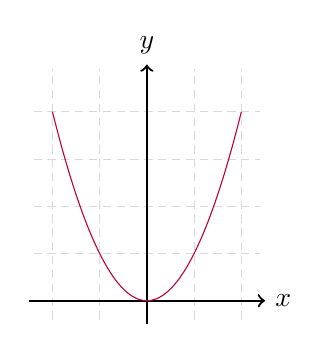
\begin{tikzpicture}[scale=0.6]
    \draw[help lines, color=gray!30,
          densely dashed] (-2.4,-0.4) grid (2.4,4.9);
    \draw[->,thick] (-2.5,0) -- (2.5,0)
          node[right]{$x$};
    \draw[->,thick] (0,-0.5) -- (0,5)
          node[above]{$y$};
    \draw[scale=1,domain=-2:2,
          smooth,variable=\x,purple]
          plot ({\x},{\x*\x});
\end{tikzpicture}
    \end{lstlisting}} &  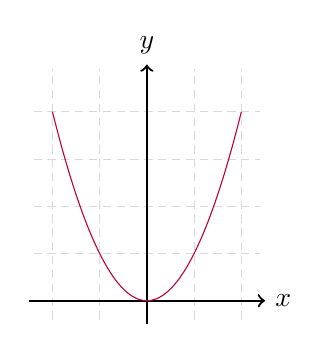
\begin{tikzpicture}[scale=0.6]
        \draw[help lines, color=gray!30,
              densely dashed] (-2.4,-0.4) 
              grid (2.4,4.9);
        \draw[->,thick] (-2.5,0) -- (2.5,0)
              node[right]{$x$};
        \draw[->,thick] (0,-0.5) -- (0,5)
              node[above]{$y$};
        \draw[scale=1,domain=-2:2,
              smooth,variable=\x,purple]
              plot ({\x},{\x*\x});
    \end{tikzpicture} &    {\footnotesize\begin{lstlisting}[style=latex,frame=none,breaklines=true]
\begin{graph}[scale=0.6,domain=-2:2]
    \plotline[purple]{\x}{\x*\x};
\end{graph}
            \end{lstlisting}}\\
    \specialrule{1pt}{0pt}{0pt}
    \end{tabular}\]
Der Befehl \CMDshow{plotline} soll hierbei nur in der Umgebung verfügbar sein (TODO: gleiches geplant mit PLA etc.).
\subsection{Positionierung}
Für die Platzierung von Plots wurden 3 valide Positionen vorgesehen: Zentriert, Links (Text auf rechter Seite), Rechts (Text auf linker Seite). Diese Positionierungen können mithilfe von Floats realisiert werden, sollen aber auf jedenfall auch noch einen absoluten Modus zur Verfügung stellen (primär von zentriert analog zu \verb|\[\]|). Zudem soll das \T{plot}-Environment selbstverständlich auch ohne Positionierung manuell eingebunden werden können!\newpage
\section{3D-Plots \LILLYxNOTExWarning{Ausstehend}}
Ich bin freier Platz :D
\renewcommand{\arraystretch}{1}
